%%%%%%%%%%%%%%%%%%%%%%%%%%%%%%%%%%%%%%%%%
% University/School Laboratory Report
% LaTeX Template
% Version 3.1 (25/3/14)
%
% This template has been downloaded from:
% http://www.LaTeXTemplates.com
%
% Original author:
% Linux and Unix Users Group at Virginia Tech Wiki 
% (https://vtluug.org/wiki/Example_LaTeX_chem_lab_report)
%
% License:
% CC BY-NC-SA 3.0 (http://creativecommons.org/licenses/by-nc-sa/3.0/)
%
%%%%%%%%%%%%%%%%%%%%%%%%%%%%%%%%%%%%%%%%%

%----------------------------------------------------------------------------------------
%	PACKAGES AND DOCUMENT CONFIGURATIONS
%----------------------------------------------------------------------------------------

\documentclass{article}

%\usepackage[version=3]{mhchem} % Package for chemical equation typesetting
%\usepackage{siunitx} % Provides the \SI{}{} and \si{} command for typesetting SI units
\usepackage{graphicx} % Required for the inclusion of images
%\usepackage{natbib} % Required to change bibliography style to APA
%\usepackage{amsmath} % Required for some math elements 
\usepackage{listings}
\lstset{
  breaklines=true,
  basicstyle=\scriptsize,
  columns=fullflexible
}

\usepackage{tikz}

\setlength\parindent{0pt} % Removes all indentation from paragraphs

\renewcommand{\labelenumi}{\alph{enumi}.} % Make numbering in the enumerate environment by letter rather than number (e.g. section 6)

%\usepackage{times} % Uncomment to use the Times New Roman font

%----------------------------------------------------------------------------------------
%	DOCUMENT INFORMATION
%----------------------------------------------------------------------------------------

\title{Report: Homework 2 - Movie Rendering Application Deployment}% Title

\author{Jan \textsc{Schlenker}} % Author name

\date{\today} % Date for the report

\begin{document}

\maketitle % Insert the title, author and date

\begin{center}
\begin{tabular}{l l}
Instructor: & Dipl.-Ing. Dr. Simon Ostermann \\
Parts solved of the sheet: & Tasks 1-6 \\
Total points: & 10
\end{tabular}
\end{center}

% If you wish to include an abstract, uncomment the lines below
% \begin{abstract}
% Abstract text
% \end{abstract}

%----------------------------------------------------------------------------------------
%	SECTION 1
%----------------------------------------------------------------------------------------

\section{How to run the programme}

First of all extract the archive file \texttt{homework\_2.tar.gz}:

\begin{lstlisting}[language=bash, deletekeywords={cd}]
  $ tar -xzf homework_2.tar.gz
  $ cd homework_2
\end{lstlisting}

Afterwards move/copy the binary files \texttt{gm} and \texttt{povray} to the \texttt{bin/} directory and the files \texttt{scherk.args}, \texttt{scherk.ini} and \texttt{scherk.pov} to the \texttt{inputdata/} directory:

\begin{lstlisting}[language=bash]
  $ cp <gm-file-path> <povray-file-path> bin/
  $ cp <scherk-files-dir>/scherk* inputdata/
\end{lstlisting}

Now you can run the the remote renderer programme:

\begin{lstlisting}[language=bash]
  $ ./myRemoteRenderer.sh user@karwendel.dps.uibk.ac.at 16 clean
\end{lstlisting}

%\begin{center}\ce{2 Mg + O2 -> 2 MgO}\end{center}

% If you have more than one objective, uncomment the below:
%\begin{description}
%\item[First Objective] \hfill \\
%Objective 1 text
%\item[Second Objective] \hfill \\
%Objective 2 text
%\end{description}

%----------------------------------------------------------------------------------------
%	SECTION 2
%----------------------------------------------------------------------------------------

\section{Programme explanation}
The files of the the programme are structured as follows:

\begin{itemize}
\item The \texttt{\textbf{myRemoteRenderer.sh}} script contains the main programme and calls \texttt{render.sh} remotely
\item The \texttt{\textbf{render.sh}} script will be copied to the remote host and basically contains homework\_1
\item The \texttt{\textbf{bin}} directory contains the binaries \texttt{povray} and \texttt{gm} which will be copied to remote host
\item The \texttt{\textbf{inputdata}} directory contains the necessary files for the \texttt{povray} binary which will be copied to remote host
\item The \texttt{\textbf{jobs}} directory contains the jobs which are executed by the \texttt{render.sh} script via \texttt{qsub} and which will be copied to remote host
\end{itemize}

The scripts and the jobs are written in shell script. One advantage of shell script for the tasks is that grid engine commands like \texttt{qsub} and \texttt{qacct} are directly available in shell script.
\\
\\
Below is the programme explanation task by task:

\begin{itemize}
% TODO: What about ssh 
\item \textbf{Task 1:} To copy all necessary files to the remote host, \texttt{my\-Remote\-Renderer\-.sh} uses \texttt{rsync}. The reason for choosing \texttt{rsync} is that the command recognizes already transfered data on the remote host.
\item \textbf{Task 2:} For rendering the files on the cluster \texttt{myRemoteRenderer.sh} calls \texttt{render.sh} on the remote host.
\item \textbf{Task 3:} To extract the job execution times the \texttt{render.sh} script stores the job\_ids and calls the \texttt{qacct} command for every job, when the rendering and merging is done.
\item \textbf{Task 4:} The \texttt{myRemoteRenderer.sh} script just uses \texttt{rsync} again to get the gif file.
\item \textbf{Task 5:} If the user passed "clean" as the third argument, \texttt{myRemoteRenderer.sh} deletes the generated files on the remote host via \texttt{ssh}.
\item \textbf{Task 6:} Figure~\ref{fig:gant} shows the execution times for an example of 64 frames rendered by 16 processors.
\end{itemize}

\begin{figure}[htbp]
\begin{center}
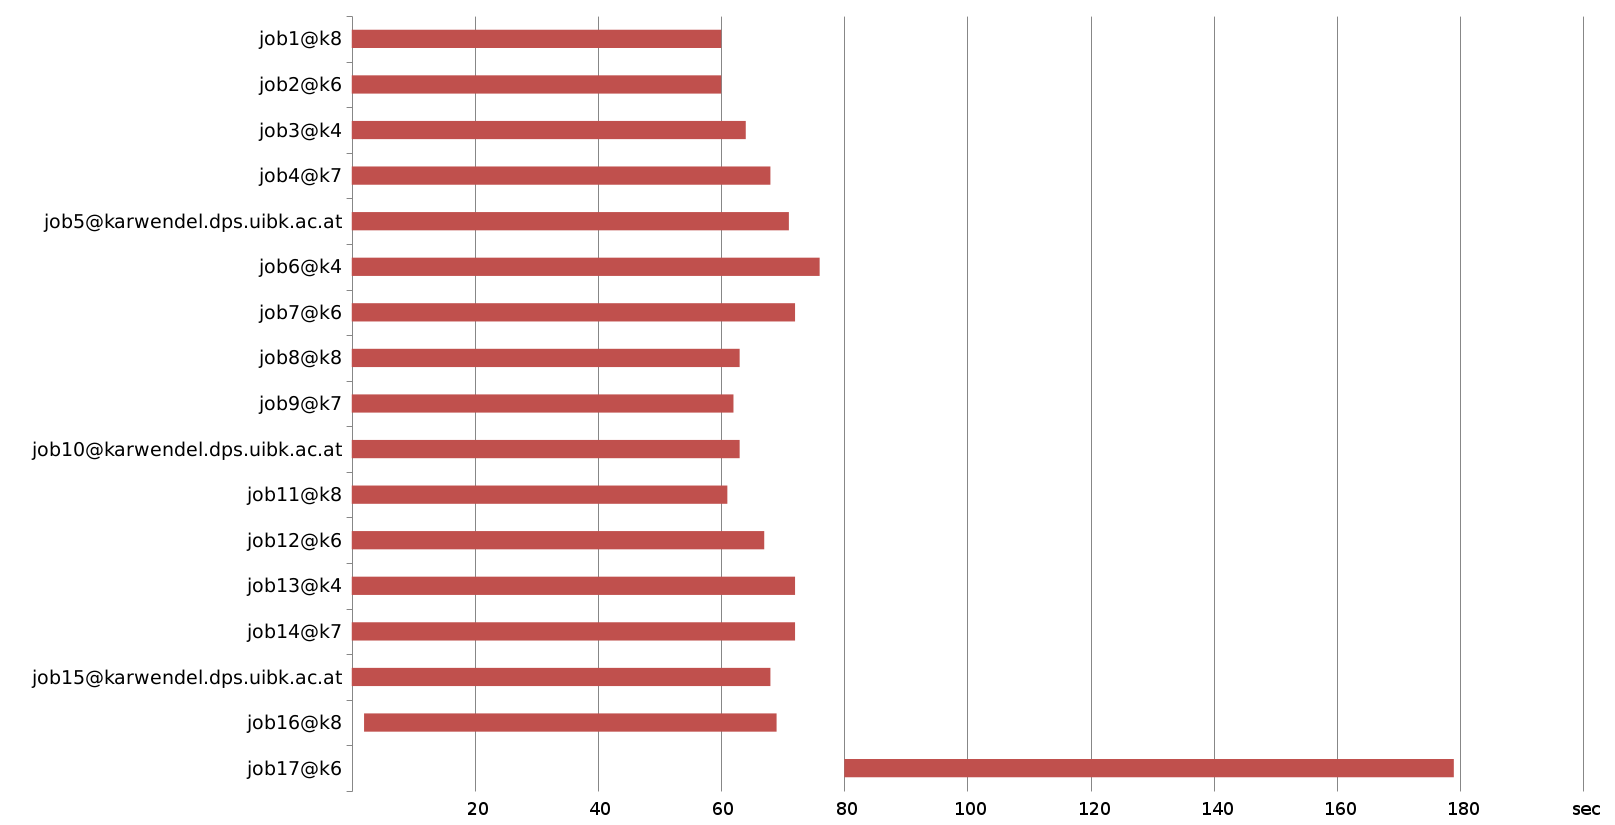
\includegraphics[width=\textwidth]{gant.png}
\caption{Gant chart for M=64 and N=16}
\label{fig:gant}
\end{center}
\end{figure}

%----------------------------------------------------------------------------------------
%	SECTION 3
%----------------------------------------------------------------------------------------

\section{Results}

The test environment consisted of a grid of 40 processors in total. 16 where used for rendering the images and 1 for merging the images. The chart shows that 16 jobs started nearly at the same time and also needed nearly the same amount of time. If we had used e.g. 70 frames instead of 64, 6 processors would propably needed more time, because 64 mod 16 = 0 and 70 mod 16 = 6. After the job rendering there is a time gap between the rendering jobs and the merger job. This can be due to shell script overhead and transfer overhead between the nodes of the grid.
\\
\\
One measurement problematic the programme has is that only the execution times given by \texttt{qacct} are considered and not the overheads. Either way the chart shows a comprehensible result.

%
%\begin{table}[htbp]
%\centering
%\begin{tabular}{ | c | p{1cm} | c | c | c | c |}
%\hline
%\textbf{Frames} & \textbf{CPUs for T$_{par}$} & \textbf{T$_{seq}$ in sec} & \textbf{T$_{par}$ in sec} & \textbf{Speedup} & \textbf{Efficency} \\
%\hline \hline
%2 & 2 & 38,15 & 23,86 & 1,60 & 0,04 \\
%\hline
%4 & 4 & 76,18 & 27,89 & 2,73 & 0,07 \\
%\hline
%8 & 8 & 147,47 & 35,90 & 4,11 & 0,10 \\
%\hline
%16 & 16 & 292,41 & 49,91 & 5,85 & 0,14 \\
%\hline
%32 & 32 & 582,99 & 75,93 & 7,68 & 0,19 \\
%\hline
%64 & 40 & 1161,30 & 141,94 & 8,18 & 0,20 \\
%\hline
%128 & 40 & 2319,09 & 277,01 & 8,37 & 0,21 \\
%\hline
%\end{tabular}
%\caption{Measurements}
%\label{tab:measurements}
%\end{table}
%

%Because of this reaction, the required ratio is the atomic weight of magnesium: \SI{16.00}{\gram} of oxygen as experimental mass of Mg: experimental mass of oxygen or $\frac{x}{1.31}=\frac{16}{0.87}$ from which, $M_{\ce{Mg}} = 16.00 \times \frac{1.31}{0.87} = 24.1 = \SI{24}{\gram\per\mole}$ (to two significant figures).

%----------------------------------------------------------------------------------------
%	SECTION 4
%----------------------------------------------------------------------------------------

%\section{Results and Conclusions}

%The atomic weight of magnesium is concluded to be \SI{24}{\gram\per\mol}, as determined by the stoichiometry of its chemical combination with oxygen. This result is in agreement with the accepted value.

%\begin{figure}[h]
%\begin{center}
%\includegraphics[width=0.65\textwidth]{placeholder} % Include the image placeholder.png
%\caption{Figure caption.}
%\end{center}
%\end{figure}
%
%----------------------------------------------------------------------------------------
%	SECTION 5
%----------------------------------------------------------------------------------------

%\section{Discussion of Experimental Uncertainty}

%The accepted value (periodic table) is \SI{24.3}{\gram\per\mole} \cite{Smith:2012qr}. The percentage discrepancy between the accepted value and the result obtained here is 1.3\%. Because only a single measurement was made, it is not possible to calculate an estimated standard deviation.

%The most obvious source of experimental uncertainty is the limited precision of the balance. Other potential sources of experimental uncertainty are: the reaction might not be complete; if not enough time was allowed for total oxidation, less than complete oxidation of the magnesium might have, in part, reacted with nitrogen in the air (incorrect reaction); the magnesium oxide might have absorbed water from the air, and thus weigh ``too much." Because the result obtained is close to the accepted value it is possible that some of these experimental uncertainties have fortuitously cancelled one another.


%----------------------------------------------------------------------------------------
%	BIBLIOGRAPHY
%----------------------------------------------------------------------------------------

%\bibliographystyle{apalike}

%\bibliography{sample}

%----------------------------------------------------------------------------------------


\end{document}
